\documentclass[aspectratio=169,10pt]{beamer}
\usetheme{Madrid}
\usecolortheme{seahorse}

\usepackage{amsmath,amssymb,amsfonts,mathtools,xcolor,listings,graphicx,hyperref}

\graphicspath{{figures/}}

\lstset{
    language=Python,
    basicstyle=\ttfamily\scriptsize,
    keywordstyle=\color{blue}\bfseries,
    commentstyle=\color{green!50!black}\itshape,
    stringstyle=\color{red},
    numbers=left,
    numberstyle=\tiny,
    frame=single,
    breaklines=true,
    showstringspaces=false
}

\setbeamertemplate{footline}[frame number]
\setbeamertemplate{navigation symbols}{}

\title{Chapter 19: Duality in Convex Optimization}
\subtitle{Convex Analysis and Monotone Operator Theory}
\author{Based on Bauschke \& Combettes (2017)}
\date{}

\begin{document}

\frame{\titlepage}

\begin{frame}{Chapter Overview}
    \begin{itemize}
        \item \textbf{19.1: Primal Solutions via Dual Solutions}
        \begin{itemize}
            \item Using dual solutions to recover primal solutions
            \item Conditions for unique primal solution
            \item Fenchel-Rockafellar duality framework
        \end{itemize}

        \item \textbf{19.2: Parametric Duality}
        \begin{itemize}
            \item Abstract dual framework
            \item Value functions and weak duality
            \item Strong duality conditions
        \end{itemize}

        \item \textbf{19.3: Lagrangian Saddle Points}
        \begin{itemize}
            \item Lagrangian function and saddle points
            \item Optimality conditions
            \item Connection to Lagrange multipliers
        \end{itemize}
    \end{itemize}
\end{frame}

\section{19.1: Primal Solutions via Dual Solutions}

\begin{frame}{The Primal and Dual Problems}
    \begin{block}{Primal Problem}
        \textbf{Minimize} $f(x) + g(Lx)$ where $f \in \Gamma_0(\mathcal{H})$, $g \in \Gamma_0(\mathcal{K})$, $L \in \mathcal{B}(\mathcal{H}, \mathcal{K})$
    \end{block}

    \begin{block}{Dual Problem}
        \textbf{Minimize} $f^*(\bullet) + g^*(\bullet)$ over appropriate dual variables
    \end{block}

    \vspace{8pt}

    \textbf{Key Questions:}
    \begin{enumerate}
        \item How are primal and dual solutions related?
        \item Can we recover the primal solution from the dual solution?
        \item When is the duality gap zero?
    \end{enumerate}
\end{frame}

\begin{frame}{Theorem 19.1: Primal-Dual Solutions}
    \begin{block}{Main Result}
        Let $f \in \Gamma_0(\mathcal{H})$, $g \in \Gamma_0(\mathcal{K})$, $L \in \mathcal{B}(\mathcal{H}, \mathcal{K})$.
        Let $x \in \mathcal{H}$, $v \in \mathcal{K}$. These are equivalent:
        \begin{enumerate}
            \item $x$ is a primal solution, $v$ is a dual solution, and $\mu = -\mu^*$
            \item $-L^* v \in \partial f(x)$ and $v \in \partial g(Lx)$
            \item $x \in \partial f^*(-L^* v) \cap L^{-1}(\partial g^*(v))$
        \end{enumerate}
    \end{block}

    \vspace{8pt}

    \textbf{Insight:} Optimality is characterized by subdifferential conditions linking the primal and dual variables.
\end{frame}

\begin{frame}{Proposition 19.4 \& 19.5: Unique Solutions}
    \begin{block}{Uniqueness via Differentiability}
        If $f^*$ is G\^ateaux differentiable at $-L^* v^*$ (where $v^*$ solves the dual), then the primal problem has either no solution or a \textbf{unique} solution:
        $$x^* = \nabla f^*(-L^* v^*)$$
    \end{block}

    \begin{block}{Projection Formula}
        When strongly convex regularization is added to the primal:
        $$\text{minimize}_x \varphi(x) + \psi(Lx - r) + \tfrac{1}{2}\|x - z\|^2$$

        If $v^*$ solves the dual, then:
        $$x^* = \text{Prox}_\varphi(z - L^* v^*)$$
    \end{block}
\end{frame}

\begin{frame}[fragile]{Example: Least Norm Problem}
    \begin{lstlisting}
import numpy as np
from scipy.optimize import minimize_scalar

# Problem: min (1/2)||x-z||^2 s.t. <a|x> = b

z = np.array([3.0, 1.0])
a = np.array([1.0, 1.0])
b = 2.0

# Closed-form dual solution
nu_star = (z @ a - b) / (a @ a)

# Recover primal solution
x_star = z - nu_star * a
mu_primal = 0.5 * np.sum((x_star - z)**2)

# Verify duality gap is zero
h_nu = lambda nu: 0.5 * (a @ a) * nu**2 + nu * (b - z @ a)
mu_dual = h_nu(nu_star)

print(f"Primal: x* = {x_star}, mu = {mu_primal}")
print(f"Dual: nu* = {nu_star}, mu* = {mu_dual}")
print(f"Gap: {mu_primal + mu_dual}")
    \end{lstlisting}
\end{frame}

\section{19.2: Parametric Duality}

\begin{frame}{Definition 19.11: Abstract Duality Framework}
    \begin{block}{General Setup}
        Given $F: \mathcal{H} \times \mathcal{K} \to [-\infty, +\infty]$:
        \begin{itemize}
            \item \textbf{Primal:} $\min_x F(x, 0)$
            \item \textbf{Dual:} $\min_v F^*(0, v)$
            \item \textbf{Value function:} $\vartheta(y) = \inf_x F(x, y)$
        \end{itemize}
    \end{block}

    where $F^*(u, v) = \sup_{x,y} (\langle x | u \rangle + \langle y | v \rangle - F(x, y))$
\end{frame}

\begin{frame}{Weak Duality (Proposition 19.12)}
    \begin{block}{The Duality Inequality}
        For any convex optimization problem:
        $$\inf_x F(x, 0) \geq -\min_v F^*(0, v)$$

        The gap between these values is the \textbf{duality gap}.
    \end{block}

    \vspace{10pt}

    \textbf{Key Points:}
    \begin{enumerate}
        \item Weak duality always holds for convex problems
        \item The dual provides a lower bound on the primal optimum
        \item The duality gap can be positive (weak duality)
        \item Or zero (strong duality)
    \end{enumerate}
\end{frame}

\begin{frame}{Strong Duality (Proposition 19.13)}
    \begin{block}{Strong Duality Condition}
        Suppose $F \in \Gamma_0(\mathcal{H} \oplus \mathcal{K})$ and the value function $\vartheta$ is lower semicontinuous at 0 with $\vartheta(0) \in \mathbb{R}$.

        Then:
        $$\inf F(\mathcal{H}, 0) = -\inf F^*(0, \mathcal{K}) \in \mathbb{R}$$
    \end{block}

    \vspace{10pt}

    \textbf{Sufficient Conditions:}
    \begin{itemize}
        \item $0 \in \text{int}(\text{dom}\, \vartheta)$ (interior)
        \item $0 \in \text{core}(\text{dom}\, \vartheta)$ (core)
        \item $0 \in \text{sri}(\text{dom}\, \vartheta)$ (strong relative interior)
    \end{itemize}
\end{frame}

\begin{frame}{Propositions 19.14 \& 19.15: Dual Solutions}
    \begin{block}{Characterization of Dual Solutions}
        The set of dual solutions is: $U = \partial \vartheta^*(0)$

        Under strong duality: $U = \partial \vartheta(0)$ and $\inf F(\mathcal{H}, 0) = -\min F^*(0, \mathcal{K})$
    \end{block}

    \vspace{10pt}

    \begin{block}{Optimality Conditions}
        For $(x, v) \in \mathcal{H} \times \mathcal{K}$, the following are equivalent:
        \begin{enumerate}
            \item $x$ is a primal solution, $v$ is a dual solution, strong duality holds
            \item $F(x, 0) + F^*(0, v) = 0$
            \item $(0, v) \in \partial F(x, 0)$
            \item $(x, 0) \in \partial F^*(0, v)$
        \end{enumerate}
    \end{block}
\end{frame}

\section{19.3: Lagrangian and Saddle Points}

\begin{frame}{Definition 19.16: Lagrangian}
    \begin{block}{The Lagrangian Function}
        $$\mathcal{L}(x, v) = \inf_y (F(x, y) - \langle y | v \rangle)$$

        A saddle point $(x^*, v^*)$ satisfies:
        $$\sup_w \mathcal{L}(x^*, w) = \mathcal{L}(x^*, v^*) = \inf_z \mathcal{L}(z, v^*)$$
    \end{block}

    \vspace{10pt}

    \textbf{Interpretation:}
    \begin{itemize}
        \item Concave in $v$ for each $x$
        \item Convex in $x$ for each $v$ (when $F$ is convex)
        \item Saddle point encodes both primal and dual optimality
    \end{itemize}
\end{frame}

\begin{frame}{Propositions 19.17-19.19: Saddle Points}
    \begin{block}{Connection to Dual Problems}
        \begin{enumerate}
            \item For convex $F$: $\sup_v \mathcal{L}(x, \mathcal{K}) = F(x, 0)$
            \item For any $v \in \mathcal{K}$: $\inf \mathcal{L}(\mathcal{H}, v) = -F^*(0, v)$
            \item Dual solution is characterized by: $\inf_w \mathcal{L}(\mathcal{H}, w) = \sup_w \inf_z \mathcal{L}(z, w)$
        \end{enumerate}
    \end{block}

    \vspace{10pt}

    \begin{block}{Complete Optimality Conditions}
        $(x^*, v^*)$ is optimal if and only if $(x^*, v^*)$ is a saddle point of $\mathcal{L}$.
    \end{block}
\end{frame}

\section{Applications}

\begin{frame}{Figures: Equality-Constrained Example}
    \begin{center}
        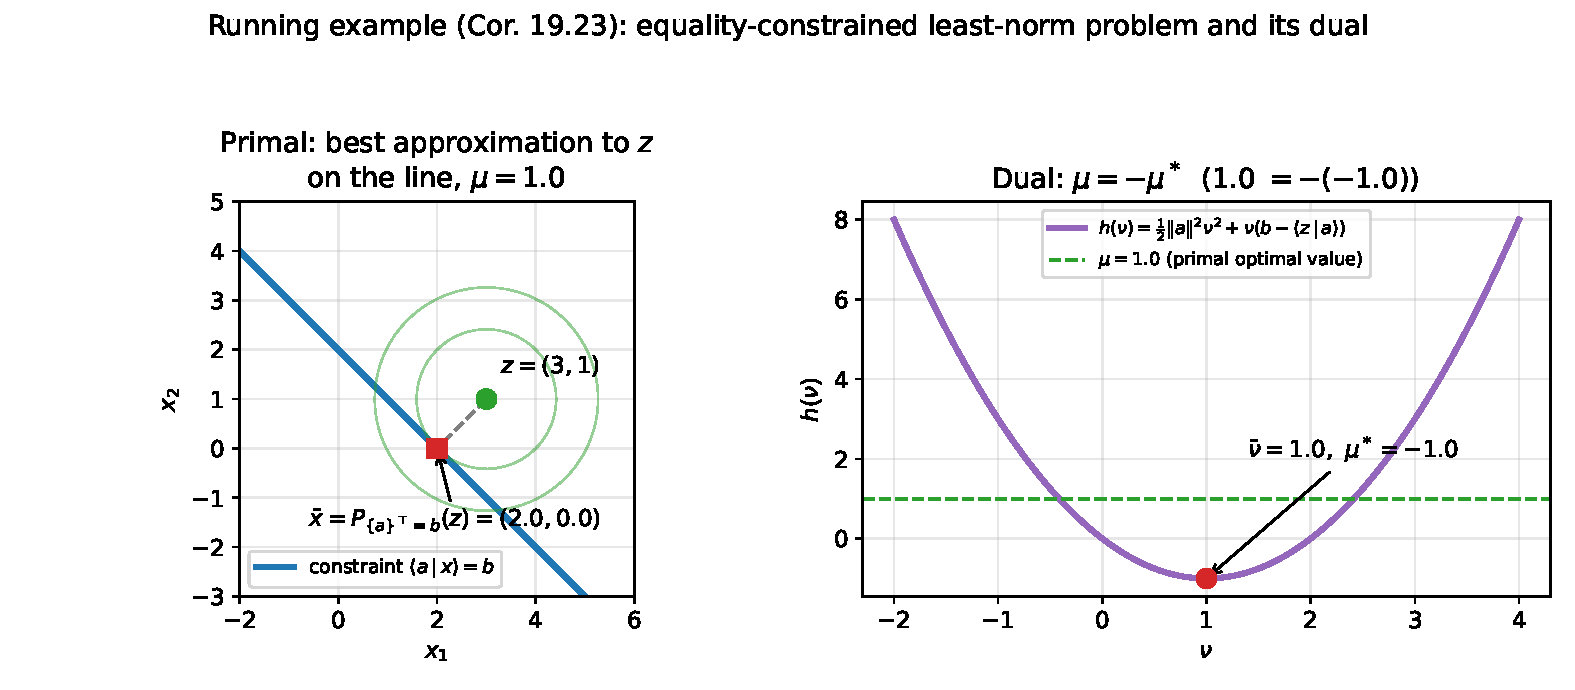
\includegraphics[width=0.95\textwidth]{fig_equality_duality}
    \end{center}

    \vspace{5pt}
    {\small Running example (Corollary 19.23): Projection onto a line.
    Left: Primal geometry; Right: Dual objective with zero duality gap.}
\end{frame}

\begin{frame}{Figures: Inequality-Constrained Example}
    \begin{center}
        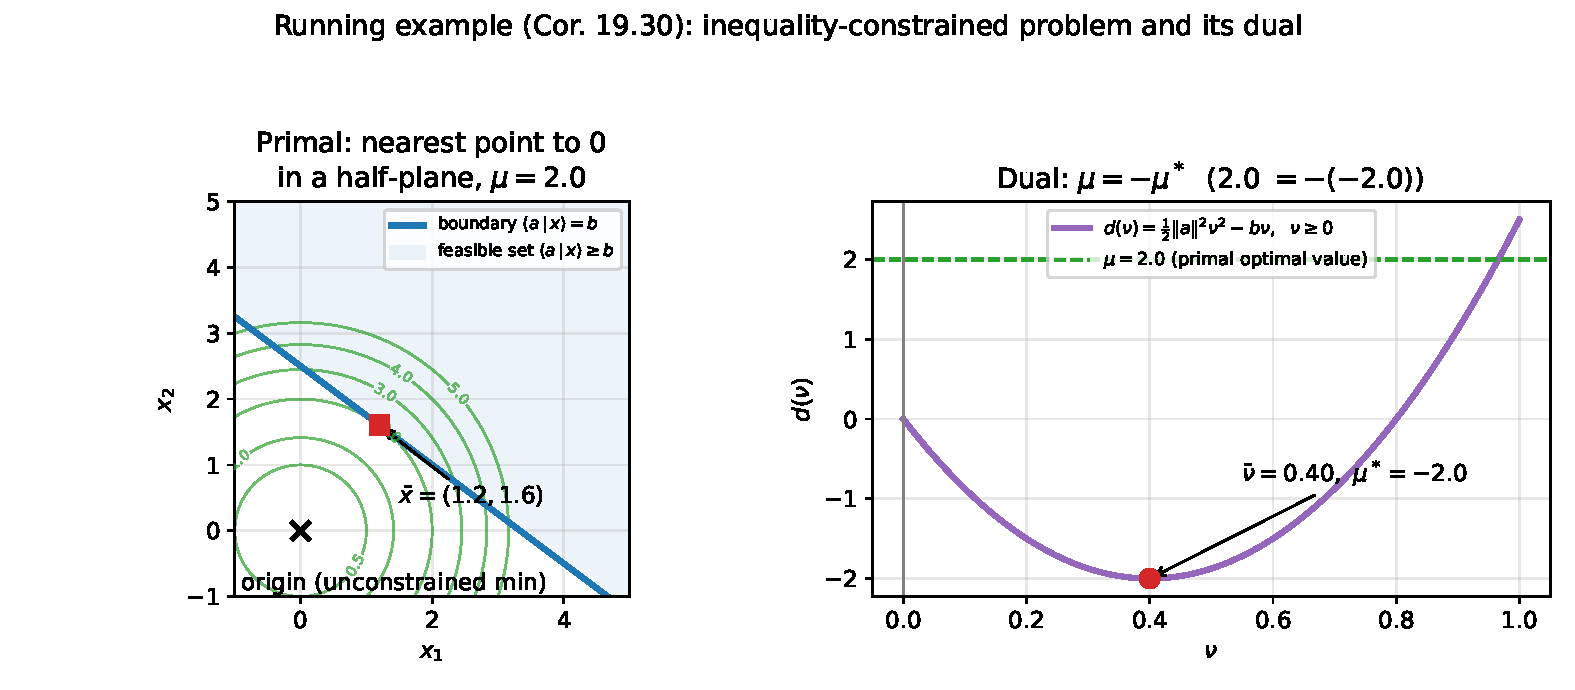
\includegraphics[width=0.95\textwidth]{fig_inequality_duality}
    \end{center}

    \vspace{5pt}
    {\small Running example (Corollary 19.30): Projection onto a half-plane.
    Left: Feasible region and optimal solution; Right: Dual objective.}
\end{frame}

\begin{frame}{Why Duality Matters}
    \begin{block}{Computational Benefits}
        \begin{enumerate}
            \item \textbf{Tractability:} Dual often easier than primal
            \item \textbf{Smoothness:} Dual objectives are differentiable (Moreau envelopes)
            \item \textbf{Decomposition:} Enables distributed/parallel algorithms (ADMM, proximal methods)
            \item \textbf{Bounds:} Dual provides lower bounds for verification
        \end{enumerate}
    \end{block}

    \vspace{10pt}

    \begin{block}{Key Applications}
        \begin{itemize}
            \item Support vector machines (SVM)
            \item Semidefinite programming
            \item Distributed optimization
        \end{itemize}
    \end{block}
\end{frame}

\begin{frame}{Key Takeaways}
    \begin{enumerate}
        \item[\textbf{19.1}] Primal solutions are uniquely recovered from dual solutions via the Fenchel-Rockafellar framework

        \item[\textbf{19.2}] Weak duality always holds; strong duality holds under regularity conditions (lower semicontinuity)

        \item[\textbf{19.3}] Lagrangian saddle points characterize optimal primal-dual pairs and connect to Lagrange multiplier theory
    \end{enumerate}

    \vspace{15pt}

    \textbf{Practical Impact:} Duality transforms difficult primal problems into more tractable dual formulations,
    enabling efficient algorithms for large-scale optimization.

    \vspace{10pt}

    \textbf{Next:} Monotone operators (Chapter 20) provide the operator-theoretic foundation for algorithm development.
\end{frame}

\end{document}
